\clearpage
\section{Forschungsteil}
\label{sec:work}

Um die Frage zu beantworten, ob es bestimmte Hänge zu einem oder dem anderen Paradigma gibt, muss zuerst beantwortet werden, wie die Paradigmen mit den Lerntypen zusammenhängen. 
Dazu wird untersucht, welche Lerntypen Vorteile beim Lernen der Computational Thinking (CT) Aspekte haben könnten. Außerdem wird geprüft, welche Empfehlungen Felder und Silverman für die Lerntypen geben und wie diese mit den Eigenschaften der Paradigmen zusammenhängen.
Hierbei wird Objektorientierung (OO) mit FP verglichen. OO wurde hier als Vergleichspunkt gewählt, da es das häufigste Paradigma in Einführungskursen der Informatik ist. FP wird betrachtet, da es den Fokuspunkt der Arbeit darstellt. Andere Programmierparadigmen werden zunächst ausgelassen.
Abschließend wird untersucht, welche Rolle die CT Aspekte in den unterschiedlichen Paradigmen spielen, um zu bestimmen, ob ein Paradigma besondere Vor- und Nachteile aufweist.

% Disclaimer
Es werden hierbei vermehrt Annahmen zu den Vorlieben der Lerntypen gemacht, aufgrund der Empfehlungen von Felder und Silvermann in Relation zu den Merkmalen der Paradigmen. Aufgrund der zeitlichen Beschränkung der Arbeit können diese Annahmen nicht empirisch überprüft werden.

\subsection{Lerntypen im Zusammenhang mit Computational Thinking}
Das Erlernen von Programmierkenntnissen umfasst nicht nur das Schreiben von Code, sondern auch den Erwerb von CT Kompetenzen.
Nicht jede Lerntypendimension zeigt Vor- oder Nachteile beim Lernen der CT Aspekte, allerdings lassen sich einige klare Zusammenhänge herausstellen.

\subsubsection{Verbal Visuell}
Visuelle Lernerinnen können einen Vorteil beim Erlernen von Abstraktion haben, da grafische Darstellungen eine sehr geeignete und beliebte Form ist, um das Konzept von Abstraktion zu erklären. Beispielsweise in der Objektorientierung werden hierbei öfters Bilder von Objekten wie Tieren oder Fahrzeugen verwendet, die dann auf Codeblöcke abstrahiert werden.
In der Informatik werden oft Vorlesungen mit starkem verbalen Input gehalten, was für verbale Lerntypen einen Vorteil bieten kann.
Zudem können visuelle Lerntypen bei der Dekomposition möglicherweise einen Vorteil, je nach Vorlesungsform haben. Ein Vorteil wäre hier möglich, wenn beispielsweise für das Aufteilen der Verantwortungen eines Klasse in der OO Programmierung grafische Darstellungen genutzt werden.

\subsubsection{Reflexiv Aktiv}
Reflexive Lernerinnen könnten einen klaren Vorteil im Aspekt Debugging haben. Sie sind eher dazu veranlagt, ihre gefundenen Lösungen zu evaluieren und zu hinterfragen. Es ist demnach wahrscheinlicher, dass ein reflexiver Lernerinnen von Natur aus Konzepte des Debugging anwendet. Aktive Lernerinnen hingegen sind risikobereiter und sind in ihrer Arbeit experimentierfreudiger. Ihr Ansatz ist es eher, schnell zu scheitern, aber auch schneller neue Lösungen auszuprobieren.

\subsubsection{Sensorisch Intuitiv}
Intuitive Lernerinnen haben einen klaren Vorteil in der Abstraktion \cite{felderhandout}. Dies ist der Fall unter anderem, da sie sich eher mit Konzepten statt Auswendiglernen beschäftigen. Sie haben oft Schwierigkeiten in Kursen, die stark auf Formelanwendung und Wiederholung setzen, und bevorzugen stattdessen neue Theorien und Interpretationen.
Auch im algorithmischen Denken werden Personen mit einem Hang zu intuitivem Lernen einen Vorteil haben, da sie normalerweise Konzepte schneller lernen als sensorische Lernerinnen. Sie ziehen Innovation den etablierten Methoden vor und meiden eher Repetition. Dies könnte im Aspekt des algorithmischen Denkens von Vorteil sein, um neue Ansätze für Probleme zu entwickeln. Besonders im Zusammenhang mit dem Aspekt des Debugging könnte diese Innovation zu schnelleren und effizienteren Lösungen führen.

\subsubsection{Sequenziell Global}
In dieser Lerndimension lässt sich ein Vorteil für sequenzielle Lerntypen im Aspekt der Dekomposition erkennen. Das Herunterbrechen auf Teilprobleme ist nicht nur ein wichtiger CT Aspekt, sondern auch eine Veranlagung des sequenziellen Lerntypen, der es vorzieht, Probleme in einem "Step by Step" Ansatz anzugehen. Sie beschäftigen sich mit allen Teilproblemen, bevor sie die komplette Lösung entwickeln können. Sequenzielle Lernerinnen können die einzelnen Teile eines Problems angehen, ohne das große Ganze zu kennen. Sie haben daher einen entscheidenden Vorteil im Herunterbrechen der Teilprobleme im Vergleich zu globalen Lerntypen.

\subsection{Eignung der Lerntypen für die Programmierparadigmen}
Nachdem die Zusammenhänge zwischen den Lerntypen und CT Aspekten untersucht wurden, muss noch betrachtet werden, inwiefern sich die verschiedenen Lerntypen für die Programmierparadigmen eignen.
Auch bei den Lerntypen des Felder Silverman Modelles lassen sich teilweise Hänge erkennen.

\subsubsection{Verbal Visuell}
Hinsichtlich der Unterscheidung zwischen visuellen und verbalen Typen lässt sich beidseitig argumentieren. Beim Erlernen von objektorientierten Konzepten wie Vererbung bieten sich visuelle Darstellungen wie Graphen an, ähnlich wie im Aspekt der CT Abstraktion.
Allerdings können visuelle Typen einfacher mathematische Konzepte und Formeln auf die Philosophien der funktionalen Programmierung übertragen und die Zusammenhänge besser verstehen. Da FP einen starken Zusammenhang mit der Mathematik hat, können durch gewohnte Strukturen von Formeln und Funktionen einfachere Parallelen gezogen werden.
Welcher Lerntyp hier einen besseren Vorteil hat, kommt allerdings sehr auf die Strukturierung der Vorlesung an.

\subsubsection{Reflexiv Aktiv}
In der aktiven und reflexiven Dimension lässt sich in beiden betrachteten Paradigmen ein Vorteil für den reflexiven Typen erkennen. Die praktische Umsetzung von Programmierkenntnissen erfolgt meistens in Einzelarbeit und erfordert eine stetige Reflexion des Lerners.
Das Erlernen von Programmierkenntnissen könnte zwar auch in Gruppenarbeiten erfolgen, aber der typische Vorlesungsstil begünstigt eher den reflexiven Lerntypen.

\subsubsection{Sensorisch Intuitiv}
In dieser Dimension lassen sich klare Präferenzen für bestimmte Paradigmen erkennen. Sensorische Typen werden höchstwahrscheinlich OO bevorzugen. Die Klassen der OO modellieren Objekte der echten Welt und haben somit einen einfach verständlichen Bezug auf echte Probleme.
Intuitive Typen hingegen sind besser darin, Abstraktion anzuwenden, und werden daher eher FP bevorzugen.
Ihr Hang zu Innvoation und abstrakteren Konzepten ohne direkten Bezug zur realen Welt bietet ihnen einen Vorteil im Verständnis und in der Umsetzung von FP.

\subsubsection{Sequenziell Global}
Auch in der sequenziell globalen Dimension lassen sich klare Zusammenhänge zu den Paradigmen erkennen. Globale Lerntypen werden es höchstwahrscheinlich vorziehen, zunächst eine OO Klasse als Ganzes zu betrachten, bevor sie sich mit der Implementierung von Details beschäftigen. Um eine sinnvolle Hierarchie zur Komposition der verschiedenen Klassen zu entwerfen, muss grundlegend ein globaleres Verständnis der Probleme vorhanden sein.
Sequenzielle Typen hingegen werden eher FP bevorzugen, da das Paradigma das Herunterbrechen von Problemen in Teilschritte von Grund auf vorsieht. Die Probleme werden in Teilfunktionen behandelt, und erst zum Schluss ergibt sich der Zusammenhang zu einem Programm. Ein globales Verständnis der Lösung ist nicht von Anfang an erforderlich.

\subsection{Ausprägung der Computational Thinking Aspekte in den Programmierparadigmen}
Um die Zusammenhänge zwischen den Vor- und Nachteilen herzustellen, muss betrachtet werden, wie genau die einzelnen CT Aspekte in den Paradigmen ausgeprägt sind. Kein Aspekt kann in einem Paradigma vollständig ausgelassen werden, da CT generell für das Konzept des Programmierens benötigt wird. Allerdings beeinflussen die unterschiedlichen Schwerpunkte und Philosophien der Paradigmen, wie die Aspekte gewertet und gewichtet werden können.
Aufgrund dieser Analyse können dann zusätzliche Schlüsse und Wichtungen der Vor- und Nachteile der Lerntypen gezogen werden.
% Hierzu wurde keine Forschung gefunden, deswegen sind das alles eigene Schlüsse (Fazitmaterial)

\subsubsection{Dekomposition}
In der FP ist die Dekomposition sehr stark ausgeprägt. Jede Funktion hat nur eine einzige Verantwortung und gibt immer dasselbe Ergebnis wieder. Durch Vermeidung von Seiteneffekten ist die Funktionsweise jeder Methode eindeutig. Der Programmablauf ist eher eine Abfolge von Befehlen als in der OO. In der OO erfolgt die Dekomposition nicht gezwungenermaßen auf Funktionsebene, sondern eher durch die einzelnen Klassen und deren Verantwortung.
\\
Da in der FP die Dekomposition einen starken Fokus hat, könnten hierbei visuelle Lerntypen eventuell einen zusätzlichen Vorteil hinsichtlich des funktionalen Paradigmas mit sich bringen, je nachdem wie die Dekomposition in der Vorlesung behandelt wird.

\subsubsection{Abstraktion}
Die Abstraktion in OO ist generell einfach zu visualisieren. Meistens werden die Probleme auf Klassen mit jeweils eigenen Funktionen heruntergebrochen. Diese Klassen wiederum können in Diagrammen oder Bildern mit ihren Funktionen dargestellt werden.
In der FP ist die Abstraktion stark mit der Dekomposition verknüpft. Um die einzelnen Teilfunktionen zu entwerfen, muss das Problem zunächst in die kleineren Einheiten zerlegt werden.
Es gibt eine sehr starke Abstraktion bis hin zu mathematischen Funktionen.
\\
Da intuitive Typen tendenziell einen Vorteil in Abstraktion haben, könnten ihnen das Erlernen von FP insgesamt leichter fallen.

\subsubsection{Algorithmen}
OO Sprachen bieten häufig ein breites Toolset für die Algorithmenentwicklung. Beispielsweise in Java sind Integer eine eigene Klasse, mit jeweils eigenen Operationen, die bei der Entwicklung verwendet werden können. In der FP hingegen ist das Toolset deutlich begrenzter, auch durch die Abwesenheit von Zuständen.
\\
Da FP stark auf innovative Lösungsansätze setzt, können intuitive Lernerinnen hier besonders profitieren.
Außerdem könnten sequenzielle Lerntypen einen zusätzlichen Vorteil in der FP haben. Die Umsetzung der Teilprobleme erfolgt isoliert voneinander und wird erst zum Schluss wieder in der Funktionskomposition zusammengesetzt. Ein globales Verständnis des Problems ist daher weniger essenziell als in der OO Programmierung.

\subsubsection{Debugging}
In der OO gibt es häufiger ein "klassisches" Debuggen. Klassen können diesen Prozess möglicherweise unübersichtlicher machen als in der FP. FP hingegen setzt stark auf Fehlervermeidung, indem Funktionen keine Seiteneffekte haben und deterministisch sind. Durch die eindeutige Verantwortung jeder Funktion treten weniger Flüchtigkeitsfehler oder unbeabsichtigte Seiteneffekte auf. Statt klassischem Debugging müssen Entwickler ständig reflektieren, und Fehler in der Funktionskomposition und in der Datenflusslogik finden.
Code in funktionalen Programmiersprachen benötigt daher generell weniger nachträgliche Bugfixes.

\begin{figure}[H]
    \centering
    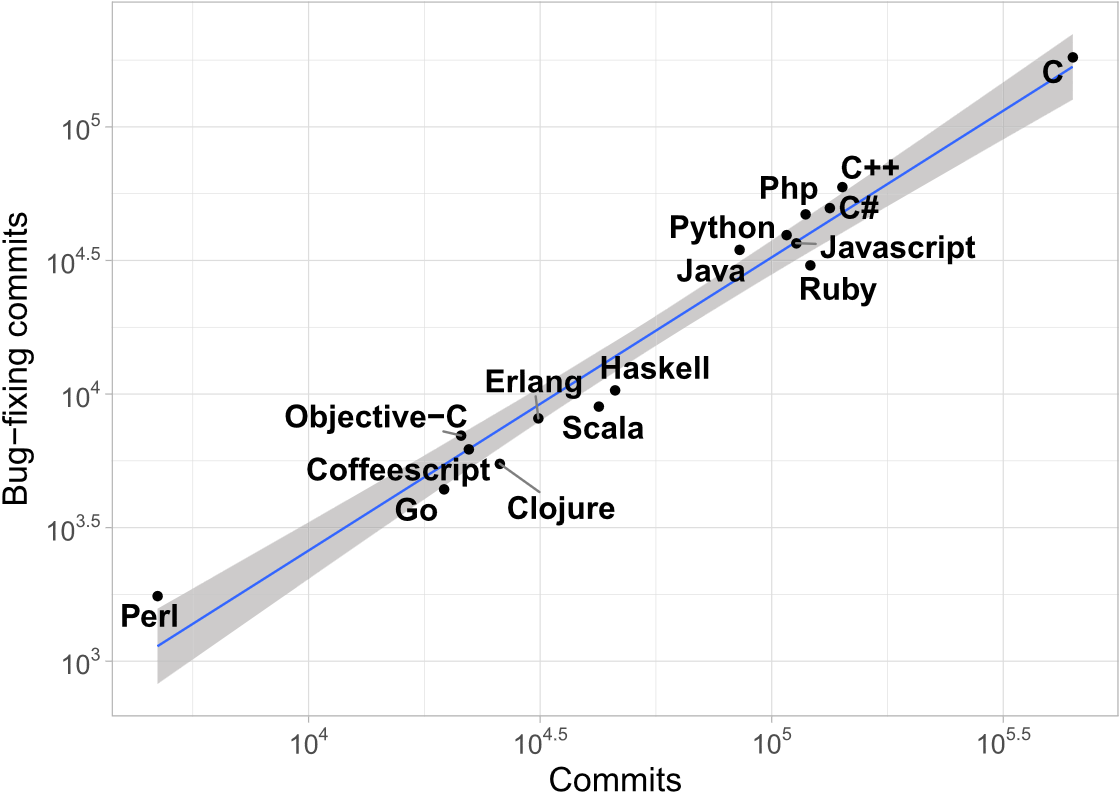
\includegraphics[width=1\linewidth]{Figures/Section_3/FigBugCommitsFP}
    \caption{Commits und Bugfixing Commits in verschiedenen Programmiersprachen \protect\cite{berger}}
\end{figure}

Aufgrund der besonders ausgeprägten Anforderung an die Reflexion beim Schreiben des Codes haben reflexive Typen möglicherweise einen zusätzlichen Vorteil in der FP.
Debugging in der FP erfordert ein abstraktes Verständnis der Vorgänge und eine ständige Reflexion der Arbeitsschritte.

\subsection{Zusammenfassung}
Zusammengefasst lassen sich also definitiv Hänge der Lerntypen zu bestimmten Paradigmen erkennen. In diesem Abschnitt werden die Vor- und Nachteile besonders im Hinblick auf die FP noch einmal übersichtlich dargestellt.

\begin{figure}[H]
    \centering
    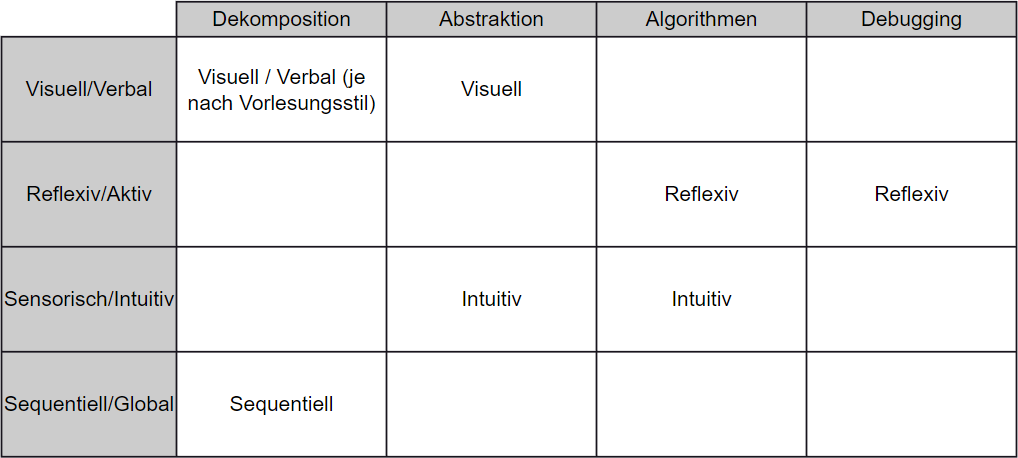
\includegraphics[width=1\linewidth]{Figures/Section_3/Styles_CT}
    \caption{Vorteile der Lerntypen in den Aspekten des Computational Thinking}
\end{figure}

Für die CT Aspekte lässt sich zusammenfassend sagen, dass besonders Personen mit visuell, reflexiv, intuitiv und sequenziell ausgeprägten Veranlagungen einen Vorteil beim Erlernen der einzelnen Aspekte haben.

\begin{figure}[H]
    \centering
    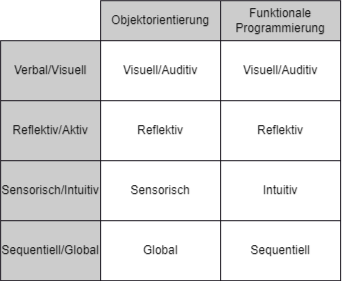
\includegraphics[width=1\linewidth]{Figures/Section_3/Styles_Paradigms}
    \caption{Vorteile der Lerntypen in den betrachteten Paradigmen}
\end{figure}

Für die Lerntypen lässt sich zusammenfassend sagen, dass besonders Personen mit reflexiv, intuitiv und sequenziell ausgeprägten Veranlagungen Vorteile beim Lernen mit funktionaler Programmierung haben.
Personen mit reflexiv, sensorischen und global ausgeprägten Eigenschaften hingegen werden besser mit OO Programmierung lernen.
Je nach Vorlesungsinhalt könnte ein visuell ausgeprägter Lerntyp noch einen zusätzlichen Vorteil in beiden Paradigmen haben.

\begin{figure}[H]
    \centering
    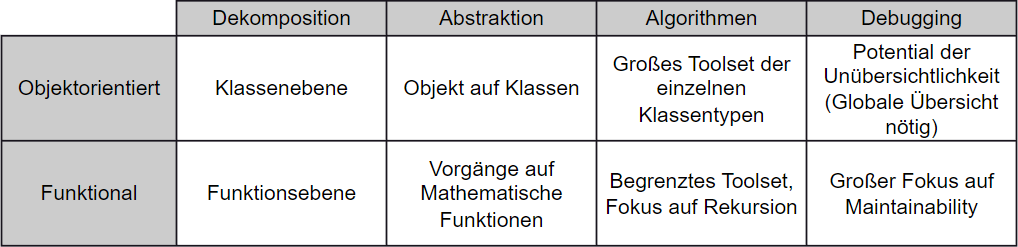
\includegraphics[width=1\linewidth]{Figures/Section_3/CT_Paradigms}
    \caption{Ausprägungen der CT Aspekte in den jeweiligen Programmierparadigmen}
\end{figure}

Zu den einzelnen Ausprägungen der CT Aspekte in den Paradigmen lassen sich zusätzliche Vorteile der Lerntypen ziehen.
Hat ein Lerntyp beispielsweise sowohl einen Vorteil beim Erlernen von algorithmischem Denken, als auch eine Neigung zu innovativen Lösungsansätzen, etwa durch eine besondere Ausprägung der intuitiven Lerntypendimension, wird dieser sich auch mit dem Toolset der FP leichter tun.

\subsubsection{Vorteile der Lerntypen in funktionaler Programmierung}
Durch die Analyse sowohl der Programmierparadigmen als auch der Computational Thinking Aspekte hinsichtlich der Lerntypen haben sich klare Vorteile einiger Ausprägungen ergeben.
Insbesondere folgende Lerntypen werden demnach Vorteile haben, wenn sie ihren Programmiereinstieg mit funktionaler Programmierung machen.

\begin{description}
    \item[Visuell] Da ein direkter Bezug zu mathematischen Formeln gemacht werden kann. Zudem haben visuelle Typen einen Vorteil in der Dekomposition.
    \item[Reflexiv] Da Programmierung tendenziell eher in Einzelarbeit erfolgt, und der Lerntyp in herkömmlichen Vorlesungsstilen besser unterstützt wird. Zudem profitiert der reflexive Typ stark durch die Fehlervermeidungsstrategie von FP. Durch ständige Reflexion der Teillösungen können potenzielle Fehler früh erkannt werden.
    \item[Intuitiv] Da dieser Typ in der FP einen besonderen Vorteil in der Abstraktion hat, die in der FP essenziell ist, da die meisten funktionalen Programmiersprachen auf dem Lambda-Kalkül basieren. Da Innovation bei neuen Algorithmen wichtig in der FP ist, hat dieser Typ auch hier einen Vorteil.
    \item[Sequenziell] Da FP einen eher sequenziell veranlagten Entwicklungsstil hat, in dem ein Teilproblem nach dem anderen angegangen wird. Zudem kann eine sequenzielle Veranlagung zusätzlich bei der Erlernung von Dekomposition helfen.
\end{description}

Diese Ausprägungen decken sich zudem mit den ausgearbeiteten Vorteilen zum Erlernen von CT Aspekten, was einen zusätzlichen Vorteil bieten kann.
\\
\subsubsection{Nachteile der Lerntypen in funktionaler Programmierung}

Andererseits haben im Umkehrschluss zum vorherigen Abschnitt wiederum folgende Lerntypen eher Nachteile bei FP.

\begin{description}
    \item[Verbal] Da verbal schwieriger ein Bezug zu den mathematischen Grundlagen von FP gemacht werden kann.
    \item[Aktiv] Da die Programmierung allgemein reflexive Typen bevorzugt. Zudem widerspricht ein aktiver Stil der Fehlervermeidung in FP, da diese eine ausführliche Reflexion der Arbeitsschritte erfordert.
    \item[Sensorisch] Da nicht so ein guter Bezug zu echten Problemen hergestellt werden kann. Zudem hat ein sensorischer Typ eher Nachteile beim Erlernen von Abstraktion und beim innovativen Ausarbeiten von neuen Lösungen für Probleme. Das Anwenden etablierter Methoden ist besonders beim Erlernen von FP schwieriger, da sich das Paradigma von anderen Programmierstilen stark unterscheidet.
    \item[Global] Da eher ein sequenzielles Denken gefordert ist. In der OO ist ein globales Denken von Vorteil, da der Zusammenhang zwischen den Domänen eine Rolle spielt und ein Verständnis der gesamten Architektur nötig ist. In der FP allerdings werden die Probleme eher schrittweise angegangen, was für diesen Lerntypen ein Nachteil sein könnte.
\end{description}